% !TEX root = main.tex

\section{数据链路层}
数据链路层把数据包,即\textbf{帧(frame)},从一个节点通过链路(直连网络或\textbf{物理网络})传给相邻另一个节点(主机和路由器)。

数据链路层的功能如下:
\begin{itemize}
	\item 成帧(framing)
	\item 差错检测(error detect):比特错,纠错
	\item 差错控制(error control):丢包、重复、错序、流控制(flow control)
	\item 介质访问控制(medium access control):多路访问,碰撞(collision)
\end{itemize}

针对点对点和多路访问网络分别制定了两个子层:
\begin{itemize}
	\item 逻辑链路控制(Logic Link Control, LLC)子层:提供可靠数据传输
	\begin{itemize}
		\item LLC1提供\textbf{无确认无连接}服务
		\item LLC2提供\textbf{有确认面向连接}的服务,实现滑动窗口协议
		\item LLC3提供\textbf{有确认无连接}的服务
	\end{itemize}
	\item 介质访问控制(Media Access Control, MAC)子层:专门用来处理多路访问网络中的冲突(点对点网络没有冲突就不用)
\end{itemize}

注意数据链路层、网络层错了就错了,不提供纠正服务,由上层纠正。
链路层在网络接口卡(network interface card, NIC)及其驱动程序上实现,路由器在接口模块上实现。

\begin{figure}[H]
	\centering
	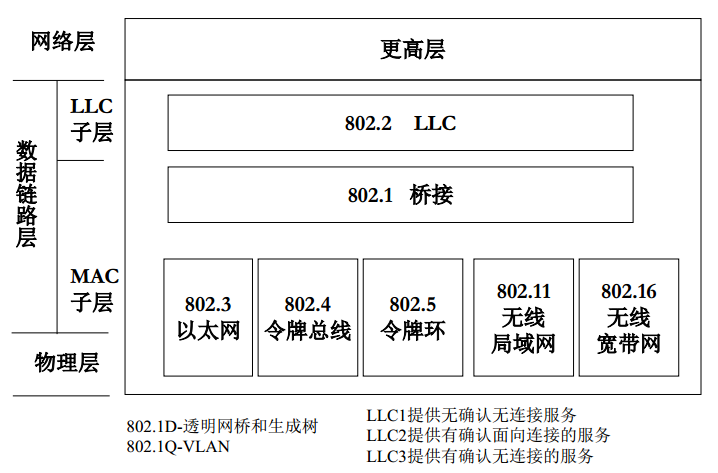
\includegraphics[width=0.6\linewidth]{fig/ieee802.PNG}
	\caption*{IEEE802系列标准}
\end{figure}

\subsection{逻辑链路控制子层}
\subsubsection{差错检测}
在数据报后加校验码(头部加序号),通过链路传输看是否有数据报/校验码错误。
\begin{enumerate}
\item 奇偶校验:若接收方收到奇数个1,则有出错
\begin{itemize}
	\item 一维偶校验:只能检错;最后补一位使得全部为偶数个1,如$010$补为$010\mid 1$,而$101$补为$101\mid 0$
	\item 二维偶校验:检错+纠错一位;横纵同时偶校验
\end{itemize}
\item 校验和(checksum):将所有数据加起来,每16位1组,最高位进位则\textbf{末尾加1},最后结果\textbf{取反}\\
由于需要使用加法器,校验和一般不用于数据链路层,而用在更高层,例如网络层和传输层
\begin{figure}[H]
	\centering
	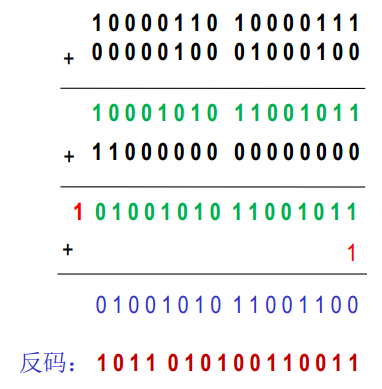
\includegraphics[width=0.4\linewidth]{fig/checksum.PNG}
\end{figure}
\item 循环冗余校验码(Cyclic Redundancy Check, CRC):
补充n位后除以一个n+1位的除数,模2除法(按位异或,做减法时没有借位)\\
接收方连带校验码一起除,余数为0则没错\\
如下图,4位除数补3个0,最后的余数011即为校验码
\begin{figure}[H]
	\centering
	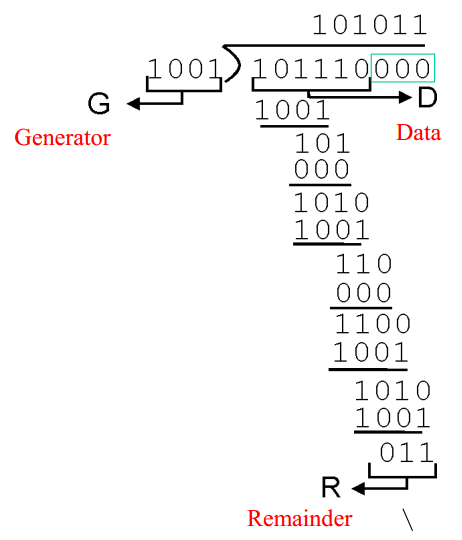
\includegraphics[width=0.4\linewidth]{fig/CRC.PNG}
\end{figure}
链路层常用CRC,因为检错率很高,且容易实现(触发器+异或门)
\end{enumerate}

\subsubsection{可靠数据传输}
每发送一帧都启动一个超时定时器,如果它的确认帧(Acknowledgement frame, ACK)在其超时时间内到达就删除该定时器;否则,自动重发请求(Automatic Repeat reQuest, ARQ)/重传该帧并重启定时器

主要的ARQ协议如下:
\begin{itemize}
	\item 停等协议(stop-and-wait):只有收到前一个数据帧的确认帧才可以发送下一个数据帧;最少需要2个序号。三种出错情况:
	\begin{itemize}
		\item 数据帧丢失(loss):正向传递时丢包
		\item 确认帧丢失:回传时丢包
		\item 超时:收到ACK表明接收方一定收到,可以发送新的数据帧,重传的也一定要发ACK
	\end{itemize}
	效率/吞吐量十分低,信道空闲时间长
	\item 滑动窗口协议(sliding window):不需等待前面发送的帧的确认帧返回,就可以连续发送下一个,其个数不能超过发送窗口大小(sending window size, SWS)\footnote{连续发送数据帧可用序号范围,用于流控制:控制发送速度,否则会发生溢出(overlow),后面覆盖前面的}\\
	这里的确认帧是指在此之前的帧都已全部收到并已交给上层协议(直连网中间没有节点,后面收到前面一定收到;只要出错纠正不了直接丢弃),后面确认前面,提高可靠性
	\begin{itemize}
	\item 回退N协议(go back N):同滑动窗口连续发送,某个ACK没收到则重传在此ACK之后的所有帧(超时重传),丢3则ACK4发2
	\begin{itemize}
		\item 发送窗口需要缓存SWS个帧,以便重传;发送窗口中序号最小的为sendbase
		\item 回退N协议可能会收到落在\textbf{发送窗口之外的确认帧},如果因确认帧迟到而出现超时重传,就可能收到一个帧的两个确认帧,第二个确认帧就会落在发送窗口之外
	\end{itemize}
	\item 选择性重传(selective repeat):通过发送否定性确认帧(negative acknowledgement, NAK)要求重传该帧;如3丢失,4发送NAK=3,5发送ACK=2,重传3
	\begin{itemize}
		\item 接收窗口(receiving window size, RWS)表示接收缓冲区大小(RWS$\leq$SWS,最好是等于,尽量减少重传帧;但序号少的话导致重复;错序到达的帧加上期待接收的帧最多SWS个),用于确定应该保存哪些帧,用序号范围表示
		\item 超时时间应该设长,确保帧的2次来回;没有后续帧也会超时重传;无论窗口内窗口外收到都要发确认
		\item 选择性重传协议可能会收到落在\textbf{接收窗口之外的数据帧},因确认帧丢失或超时到达而重传的数据帧都会落在接收窗口之外
		\item 选择性重传协议丢失了NAK并非致命错误,因为还有超时重传机制,保证该数据帧能够重新发送
	\end{itemize}
	\end{itemize}
\end{itemize}
\par ARQ协议的超时时间不应设置得太长,否则会导致系统需要花很长的时间来纠正这些错误;ARQ设得短可以使查出错误的时间变短,同时提升网络的吞吐量(但也不能设太短,否则发送方会大量误认为帧丢失而产生不必要重传)。

% 如果当前RTT=1ms,采用选择性重传(selective repeat)滑动窗口协议,超时时间应设置为略大于2ms;如果收到NAK就重置所有的超时定时器,那超时时间应设置为略大于1ms。
% 这里假设收到NAK的重传不重置超时定时器,否则,一个RTT也可以。

注意不管哪一种重传机制,序号可以重复使用,因此有最小序号问题。
\begin{example}
	序号8个,SWS=RWS=4,345670123456,5丢失
\end{example}
\begin{analysis}
	回退N:346705670123456\\
	选择性重传:346705123456
\end{analysis}
\begin{example}
	把停等协议用于一个带宽为20Mbps、长度为3000公里、传播速度为200000公里/秒的点到点链路,如果最长帧为5000字节,带宽的最大利用率(最大吞吐量/带宽)是百分之多少?
\end{example}
\begin{analysis}
	按照如下方法计算
	\begin{itemize}
		\item 传播延迟$RTT$:$(3\times 10^6 m) / (2\times 10^8 m/s)\times 2=30ms$(注意是\textbf{往返时间}!)
		\item 传输延迟$L/R$:$(5000B\times 8)/(20\times 10^6bps)=2ms$
		\item 吞吐量:$L/(RTT+L/R)=(5000B\times 8)/32ms=1.25Mbps$
		\item 带宽最大利用率:最大吞吐量/带宽=$1.25/20\times 100\%=6.25\%$
	\end{itemize}
	另,改为滑动窗口协议,窗口大小为8,则最大利用率位$8\times 6.25\%=50\%$
\end{analysis}

提高滑动窗口协议的效率:
\begin{itemize}
	\item 选择性确认(selective acknowledgement):接受方把已收到的帧的序号告诉发送方(收到不用重传告诉发送方哪些已收到,则只用重传某帧)
	\item 捎带确认(piggybacking):通信双方\textbf{全双工}方式工作,接收方在发数据给对方时顺便把确认号也告诉对方(两个滑动窗口,两边都要发数据),需要结合下面一起使用
	\item 延迟确认(delayed acknowledgement):接收方收到一帧后并不立即发送确认帧,而是等待一段时间再发送
\end{itemize}

\subsection{介质访问控制子层}
\subsubsection{简介}
\begin{enumerate}
\item \textbf{PPP协议(point-to-point):点对点网络}
\begin{itemize}
	\item 根据HDLC(high-level data link control)协议进行设计,主要用于串行电缆、电话线(MODEM)等串行链路
	\item 提供连接认证、传输加密和压缩功能,为网络层协议提供服务
	\item 采用字节填充法(byte-stuffing)替换掉保留字
	\item 没有纠错功能,也没有流控制和确保有序的功能
	\begin{figure}[H]
		\centering
		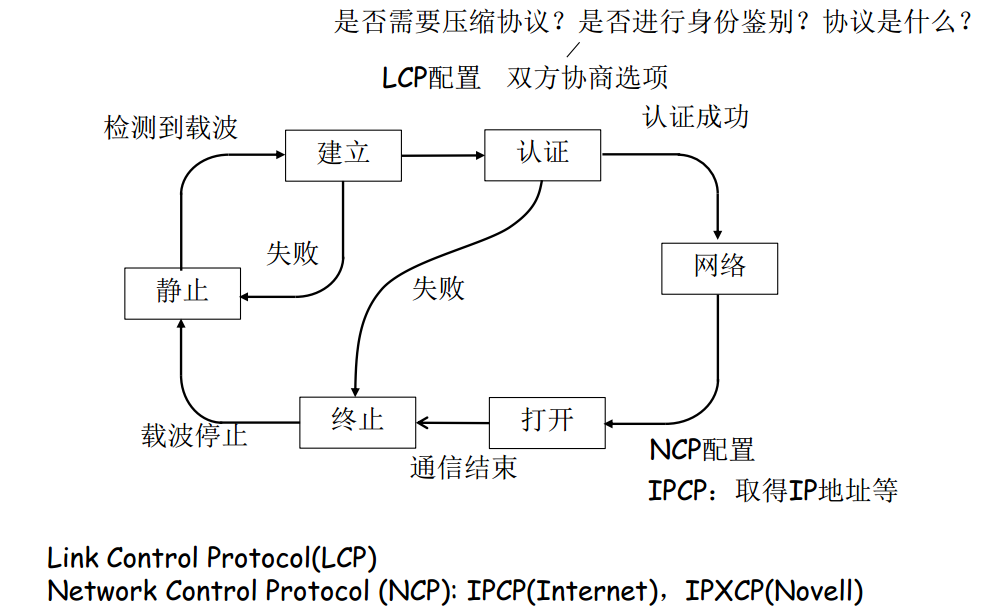
\includegraphics[width=0.6\linewidth]{fig/PPP.PNG}
	\end{figure}
\end{itemize}

\item \textbf{以太网:多路访问网络}\\
解决冲突问题:随机访问协议(random access protocol),注意不是滑动窗口不用发确认帧
\begin{itemize}
\item 纯ALOHA:想发送就发送,超时未收到确认则发生冲突
\item 分槽ALOHA:将时间分为长度相同的时槽,每个站点只在时槽开始时发送。\\
信道空,立即以概率$p$发送,以概率$1-p$延迟一个时间槽;信道忙,延迟一个时间槽。
\item 载波监听CSMA(Carrier Sense Multiple Access):发送前先监听信道
\begin{itemize}
	\item 信道空,立即发送;信道忙,持续监听(1-persistent CSMA,以太网)
	\item 信道空,发送;信道忙,延迟一段随机长度时间(non-persistent CSMA),较省电
	\item 信道空,立即以概率$p$发送,以概率$1-p$延迟一个时间槽;信道忙,延迟一个时间槽(p-persistent CSMA,分槽ALOHA)
\end{itemize}
\end{itemize}
\end{enumerate}

\subsubsection{以太网物理层协议}
IEEE 802.3规定以太网物理层标准:
\begin{itemize}
	\item 传输方法:均使用\textbf{异步传输},即信道空闲时以太网设备不任何发送信号
	\item 编码方法:曼彻斯特编码
	\item 命名规则: 10BaseT的10表示10Mbps,Base表示基带传输,T表示双绞线;10base2的2表示最大距离200m
\end{itemize}
与802.3相比,快速以太网(100BaseTX)只是把传输速率提高到100Mbps
\begin{itemize}
	\item MAC子层的协议不变:CSMA/CD协议不变,帧格式不变
	\item 最大距离改为100m (10base5的最大距离为2500m),物理层改动
	\item 帧间空隙隔依然为96b,即$0.96\mu s$
\end{itemize}

集线器(hub)采用电子线路方法模拟总线方式的以太网,两台主机同时发送会产生冲突,所以是\textbf{半双工}工作。
如果通过两个接口同时发送数据会产生冲突,则这两个接口属于同一个冲突域(collision domain)。一个广播帧可以到达的所有接口属于同一个广播域。
属于同一个冲突域的以太网部分称为网段(segment)。
\begin{example}
	下图的冲突域和广播域个数?
	\begin{figure}
		\centering
		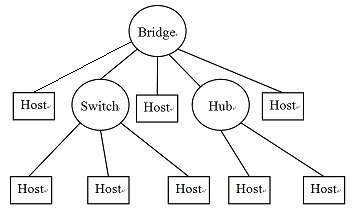
\includegraphics[width=0.35\linewidth]{fig/conflict_count.jpg}
	\end{figure}
\end{example}
\begin{analysis}
交换机(switch)/网桥(bridge)的每个端口处于一个冲突域,集线器(hub)的所有端口处于一个冲突域。故8个冲突域,1个广播域。
\end{analysis}

集线器、交换机、路由器区别见\ref{subsub:physical_equipment}节。

\subsubsection{以太网MAC层协议}
以太网采用帧间空隙(interframe space)的成帧方法(每帧发送前要求信道空闲时间至少为96bits,造成每帧之间有空隙)。
采用载波监听CSMA/CD(with collision detection)协议(1-坚持CSMA)。
\begin{enumerate}
	\item 发送数据帧之前先监听信道。如果信道空闲,\textbf{立即}发送。
	如果信道忙,则\textbf{持续监听},直到信道空闲,立即发送。
	\item \textbf{边发送边检测}冲突。如果发送完毕都没有检测到冲突,则发送成功。
	\item 如果检测到冲突,则\textbf{停止发送},并发送32位干扰位(jamming signal)以加强冲突信号。
	采用二进制指数退避算法\textbf{随机延迟}一段时间后,转(1)。
\end{enumerate}

二进制指数退避算法(binary exponential backoff)
\begin{itemize}
	\item 规定最短帧是为了使发送站点可以监测到所有冲突,选择最短帧的发送时间作为其时间槽(time slot)$\tau$的长度,最短帧的发送时间保证了首先发送的站点的信号可以到达最远的站点。如果先发送的只有一个站点,其他站点要不就检测到发送站点的信号而不能发送,要不就因为发送站点发送完毕而检测到信道空闲,总之不会与之冲突。也就是说,任何间隔$\tau$或以上时间的两个发送数据的站点不会发生冲突。
	\item 时间片$\tau$的长度为512b时间,10Mbps的以太网为51.2$\mu s$
	\item 第$i$次冲突从$0,1,\ldots,2j-1$个时间片随机选择一个,$i<16$,$j = min(i,10)$
	\item 前十次冲突后可选时间片数量每次加倍,后五次冲突后可选时间片数量不变,所以也称	为截止式(truncated)二进制指数退避算法
\end{itemize}
\begin{example}
	当一个以太网的信道忙时有五个站点都想发送一个最长帧(长度为1520B),如果很长时间只有这五帧要发送,问最少经过几次冲突就可以全部发送成功?
\end{example}
\begin{analysis}
	最长帧占用$1520B\times 8/512b=23.75$个时间槽,而在第1、2、3、4次冲突的延迟时间最多16个时间槽,首先发送的站点都会引起后续所有站点冲突。
	最好情况每次冲突后都让一个站点发送成功,所以最少4次冲突。
	详细来说,一开始5个站点同时发送,第一次冲突,随机延迟0或1个时间片,假设0号立即发送,其他4个延后1个时间片,那么0号发送成功,其他4个检测到信道忙,不发送。
	到0号发完时,信道空闲,其他4个同时发送,第二次冲突,如此类推,每次成功发送一个。
\end{analysis}

802.3的MAC帧格式
\begin{center}
前导字符(8B)+目的地址(6B)+源地址(6B)+类型/长度(2B)+有效载荷/填充位+帧校验序列(4B)
\end{center}
\begin{itemize}
\item 源地址:一般为发送者的单播地址
\item 目的地址(6B):一般为接收者的单播地址
\end{itemize}

MAC地址
\begin{itemize}
	\item 单播/网卡/烧录地址:全球唯一,每个网卡/接口一个
	\item 多播地址:字节0第0位为1,地址非全1
	\item 广播地址:48位全为1
\end{itemize}

\subsubsection{透明网桥}
透明网桥的三个操作:
\begin{itemize}
	\item 表里查到则\textbf{转发}(forward)
	\item 表里没有则扩散/\textbf{泛洪}(flood):由端口P1,扩散到其他所有端口P2,P3(多播、广播一定扩散)
	扩散不回传
	% 只要广播都要收下了,操作系统一定要处理
	收到的部分不会往回转
	\item 从某一条路发来则不能传回去,过滤/\textbf{丢弃}(filter)
\end{itemize}

透明网桥有自学习机制:利用\textbf{源地址}学习,如信息从A主机-P1端口来,则记为A-P1,同时设好生存期(Time to live, TTL)\footnote{单位为秒,每次发送都会重置,对于不活跃的表项自动删掉(减少表的大小,查找速度更快)}。
如果收到的帧有错则直接丢弃,根本不会学习。
如果源地址已经在表中,则更新记录,并重置超时计时器。

扩展/桥接局域网:每一个局域网(LAN)都是一个网段
\begin{example}
	下面的扩展LAN包含三个透明网桥B1、B2、B3和四台主机A、C、D、E。
	如果网桥的MAC地址表初始都是空的,在以下三次传输之后MAC地址表的内容是什么?
	\begin{enumerate}
	\item D发送了一个帧给E
	\item A发送了一个帧给D
	\item C发送了一个帧给A
	\end{enumerate}
	\begin{figure}[H]
		\centering
		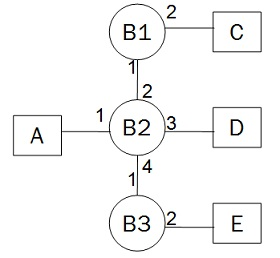
\includegraphics[width=0.3\linewidth]{fig/mac_address.jpg}
	\end{figure}
\end{example}
\begin{analysis}
	\begin{minipage}{0.32\linewidth}
	\begin{table}[H]
		\centering
		\caption*{B1的MAC地址表}
		\begin{tabular}{|c|c|}\hline
			MAC地址 & 端口 \\\hline
			D & 1\\\hline
			C & 2\\\hline
		\end{tabular}
	\end{table}
	\end{minipage}
	\begin{minipage}{0.32\linewidth}
	\begin{table}[H]
		\centering
		\caption*{B2的MAC地址表}
		\begin{tabular}{|c|c|}\hline
			MAC地址 & 端口 \\\hline
			D & 3\\\hline
			A & 1\\\hline
			C & 2\\\hline
		\end{tabular}
	\end{table}
	\end{minipage}
	\begin{minipage}{0.32\linewidth}
	\begin{table}[H]
		\centering
		\caption*{B3的MAC地址表}
		\begin{tabular}{|c|c|}\hline
			MAC地址 & 端口 \\\hline
			D & 1\\\hline
		\end{tabular}
	\end{table}
	\end{minipage}
\end{analysis}

之所以称为透明,是因为插入网桥后无需改动硬件和软件,也无需设置地址开关、装入路由表或参数等,网桥就能工作(自学习)。

\subsubsection{生成树协议}
将所有的LAN和网桥都抽象为结点,避免冲突即构造一棵生成树(注意不是最小生成树)
\begin{itemize}
\item IEEE 802.1D 生成树协议+透明网桥
\item IEEE 802.1w RSTP(Rapid Spanning Tree Protocol)
\end{itemize}

工作流程如下
\begin{itemize}
\item 先确定根网桥,即\textbf{BID(Bridge ID)最小}的
\item 每个网段(需要集线器)依赖于连通的网桥,每个网桥都把自己到根的距离发出去(竞选/配置消息)
\item 网桥之间的开销为1,选一条\textbf{最短路径}
\item 扩散自己BID,最后只剩下根网桥认为自己是根
取得优胜的,作为指定网桥;相同距离时,BID小的优胜;端口号小的优胜
\item 网桥只在根端口和指定端口之间转发\textbf{数据}帧,不可通过阻塞端口
\item 只有从根端口过来的才扩散配置消息,其他端口来的不扩散,这样不会形成回路
\item 断了/失效了则变成无穷大,其他网桥可成为指定网桥
\end{itemize}

防止广播风暴,又能自动修复损害网桥(通过冗余方式),增加可靠性
\begin{example}
	下图显示了由五个透明网桥(B1~B5)形成的扩展LAN。
	\begin{figure}[H]
		\centering
		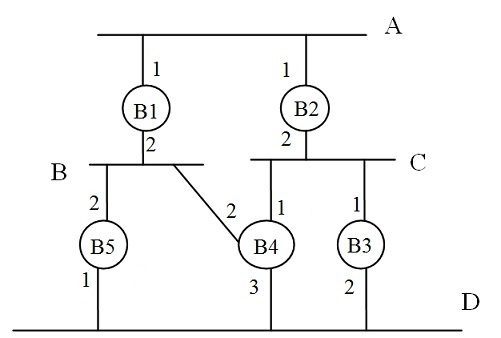
\includegraphics[width=0.4\linewidth]{fig/bridge.jpg}
	\end{figure}
\end{example}
\begin{analysis}
\begin{enumerate}
	\item B1是根网桥
	\item 网段A-D的指定网桥(designated bridges)分别是
\begin{center}
	\begin{tabular}{|c|c|c|c|}\hline
		A & B & C & D\\\hline
		B1 & B1 & B2 & B4\\\hline
	\end{tabular}
\end{center}
\item 网桥B1-B5的根端口分别是
\begin{center}
	\begin{tabular}{|c|c|c|c|c|}\hline
		B1 & B2 & B3 & B4 & B5\\\hline
		无 & 1 & 1 & 2 & 2\\\hline
	\end{tabular}
\end{center}
\end{enumerate}
\end{analysis}

\begin{example}
	下图是一个扩展LAN:
	\begin{figure}[H]
		\centering
		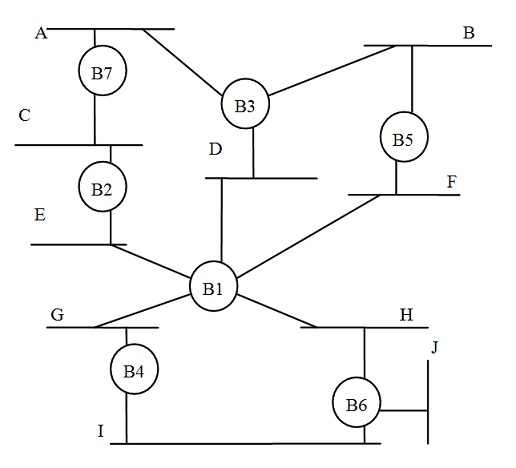
\includegraphics[width=0.4\linewidth]{fig/spanning_tree.jpg}
	\end{figure}
\end{example}
\begin{analysis}
	\begin{itemize}
		\item[a.] 如果B1没有启动生成树算法但是转发生成树消息(BPDU),只生成1棵生成树,根为B2
		\item[b.] 如果B1没有启动生成树算法而且丢弃所有收到的生成树消息(BPDU),生成2棵生成树,根分别为B2和B4
	\end{itemize}
\end{analysis}

\subsubsection{虚拟局域网}
虚拟局域网(Virtual LAN, VLAN)将原来的局域网分割成多个相互隔离的局域网,只在具有相同颜色的端口间转发。

如果所有交换机都是连通的,并且交换机连至交换机的接口都配置为trunk接口,交换机连至主机的接口都配置为VLAN接口(主机接口),则所有连至相同的VLAN接口的主机都位于同一个广播域,连至不同VLAN接口的主机位于不同的广播域。

每次扩散扩散到帧内指定的端口或\textbf{干道端口},同样查MAC地址表转发。
只有发往干道端口的帧才需要加上VLAN ID。
如果从干道收到的帧没有VLAN ID,则认为是本征(native)VLAN,默认为VLAN1。
\begin{example}
	下图中哪些发送的帧将被目的主机收到
	\begin{figure}[H]
		\centering
		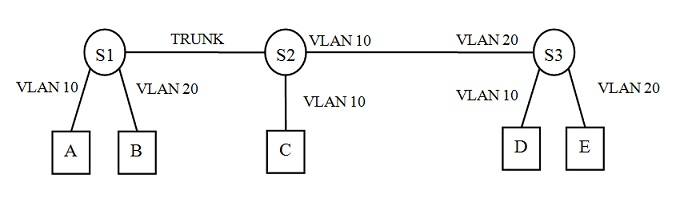
\includegraphics[width=0.5\linewidth]{fig/vlan.jpg}
	\end{figure}
\end{example}
\begin{analysis}
	只有A到E或E到A可以成功发送信息,注意S2和S3的端口设错了(故意的)。
	如E到A,VLAN20经过S3转发到VLAN20,发到S2。
	S2误认为是从VLAN10发来的消息,故扩散到干道端口TRUNK加VLAN10,发到S1。
	S1接收到后转发至VLAN10。\\
	而D到B没有办法,因为从S3就转发不出去,没有干道端口。
\end{analysis}

多生成树协议:管理员规定哪些VLAN为一组,构成多生成树,其余的用公共生成树
\begin{itemize}
	\item 公共生成树(common spanning tree, CST)
	\item 多生成树(Multiple spanning tree protocol, MSTP)
\end{itemize}

\subsubsection{令牌环网}
令牌环网(token ring):通过在站点之间传递令牌防止冲突并且具有
\textbf{优先权}的星形\textbf{LAN},其标准为IEEE 802.5,take turns protocol,现在有千兆令牌环网。
多站点接入部件称为(multistation access unit, MSAU)
\begin{figure}[H]
	\centering
	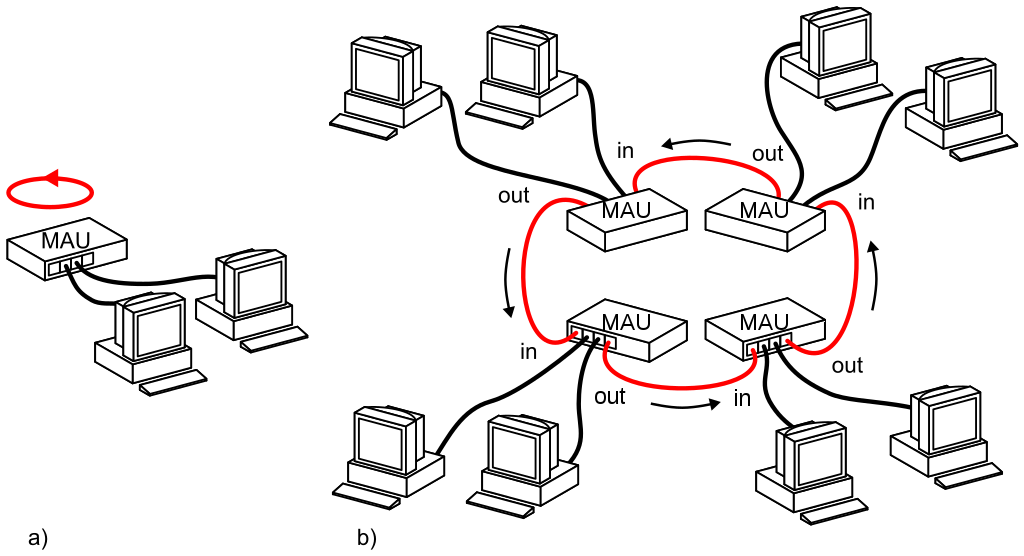
\includegraphics[width=0.5\linewidth]{fig/token-ring.png}
\end{figure}

数据传送过程:
\begin{itemize}
	\item 令牌(帧)绕环而行
	\item 只有截获令牌的站点才可以发送数据帧,各站点保有令牌帧的时间是相同的
	\item 发送的数据帧通过所有的活动站点
	\item 目的站点拷贝数据帧
	\item 只有发送方移除数据帧
	\item 当没有数据帧要发送或者持有时间到,当前的发送站点要释放令牌;被释放的令牌继续绕环而行
\end{itemize}

注意:以太网没有确认机制,没有优先权。
必然有特殊的站点(监控站点)产生令牌帧,选举出监控站点(MAC地址最小)。

源路由桥接算法:由IBM开发的用于令牌环网的协议,将路径记到头部,下一次就不用查。
为了兼容普通交换机,源路由网桥交换机也必须实现透明网桥的功能。

\subsubsection{物理设备}
\label{subsub:physical_equipment}
交换机是一个把多个网段连接起来的设备,也称为\textbf{多端口网桥}(switch=bridge)。
注意输入输出端口一样。

交换结构(fabrics)
\begin{itemize}
	\item 共享总线式交换机:同样有冲突问题
	\item 纵横式(crossbar)
\end{itemize}

交换机转发方法
\begin{itemize}
\item 存储转发(store and forward):交换机收到整个帧后转发\\
目的MAC地址(6B),转也要依照CSMA/CD来转发
\item 直通(cut through):收到一个转一个,出现碎片
\item 无碎片(fragment free):都没冲突才开始转发,\textbf{最小帧保证}\\
交换机不用收到整个帧而是收到64B(冲突窗口)后自动转发
\item 适应性交换(adaptive switching):自动在上面三种方式中选择
\end{itemize}

交换机的工作模式
\begin{itemize}
\item 全双工模式:因为没有冲突,CSMA/CD算法可以被关闭
\item 自动翻转(auto-MDIX):
大部分交换机可以自动选择连接方式,\textbf{交叉线}或\textbf{直通线}
\item 自适应(autonegotiation):两个站点周期性使用快速链路脉冲(fast link pulse,FLP)选择10M/100M/1000Mbps自适应
\end{itemize}

% 如果主机A发送IP分组给主机B, 主机B收到的帧中的源地址是什么?
% 连接模式: [host A]--[Router R1]--[Router R2]--[host B],其中包含3个以太网。
% R2的MAC地址

集线器、交换机、路由器的区别如下\footnote{\url{http://www.qianjia.com/html/2017-08/09_274208.html}}:
\begin{itemize}
	\item 集线器(hub):\textbf{物理层/一层},广播,排队,冲突,共享型设备(一个端口往另一个端口发数据,其他端口就处于等待状态),半双工,监听,响应
	\item 交换机(switch):\textbf{数据链路层/二层},MAC地址,建立连接,独享信道,全双工,增加冲突域数量,减少冲突范围大小
	\item 路由器(router):\textbf{网络层/三层},建立路由表,IP地址,路由选择
\end{itemize}

路由器与其他两者的区别:
\begin{enumerate}
\item 集线器工作在第一层,没有智能处理能力,对它来说,数据只是电流,当一个端口的电流传到集线器中时,它只是简单地将电流传送到其他端口,至于其他端口连接的计算机接收不接收这些数据,它就不管了。
交换机工作在第二层,它要比集线器智能一些,对它来说,网络上的数据就是MAC地址的集合,它能分辨出帧中的源MAC地址和目的MAC地址,因此可以在任意两个端口间建立联系,但是交换机并不懂得IP地址,它只知道MAC地址。
路由器工作在第三层,它比交换机还要更智能一些,它能理解数据中的IP地址,如果它接收到一个数据包,就检查其中的IP地址,如果目标地址是本地网络的就不理会,如果是其他网络的,就将数据包转发出本地网络。

\item 路由器能连接不同类型的网络,我们常见的集线器和交换机一般都是用于连接以太网的,但是如果将两种网络类型连接起来,比如以太网与ATM网,集线器和交换机就派不上用场了。
路由器能够连接不同类型的局域网和广域网,如以太网、ATM网、FDDI网、令牌环网等。
不同类型的网络,其传送的数据单元---帧的格式和大小是不同的,数据从一种类型的网络传输至另一种类型的网络,必须进行帧格式转换。
路由器就有这种能力,而交换机和集线器就没有。
而互联网就是由各种路由器连接起来的,因为互联网上存在各种不同类型的网络,集线器和交换机根本不能胜任这个任务,所以必须由路由器来担当这个角色。

\item 路由器具有路径选择能力,在互联网中,从一个节点到另一个节点,可能有许多路径,路由器可以选择通畅快捷的近路,会大大提高通信速度,减轻网络系统通信负荷,节约网络系统资源,这是集线器和二层交换机所根本不具备的性能。
\end{enumerate}

小范围的局域网,如我们的校园网大多采用交换机,路由少。